% Quelle: https://tex.stackexchange.com/questions/124144/fill-of-a-thermometer
\PassOptionsToPackage{dvipsnames}{xcolor}
\documentclass[letterpaper,tikz,convert=false]{standalone}
\usepackage{fourier}
\usepackage{pxfonts}
\usepackage{units}
\usepackage{tikz, pgf}

\tikzset{
  thermometer/.style={insert path={
    (280.0313,169.3125) .. controls (263.9888,169.3125) and (250.6461,179.3446) ..
    (247.8125,192.5625) -- 
    (247.3438,563.7500) .. controls (235.7346,573.2243) and (228.3438,587.6282) ..
    (228.3438,603.7813) .. controls (228.3438,632.3161) and (251.4651,655.4688) ..
    (280.0000,655.4688) .. controls (308.5349,655.4688) and (331.6563,632.3161) ..
    (331.6563,603.7813) .. controls (331.6563,587.6282) and (324.2654,573.2243) ..
    (312.6563,563.7500) -- 
    (312.2500,192.5625) .. controls 
    (309.4164,179.3446) and (296.0737,169.3125) .. (280.0313,169.3125) -- cycle
}}}
\begin{document}
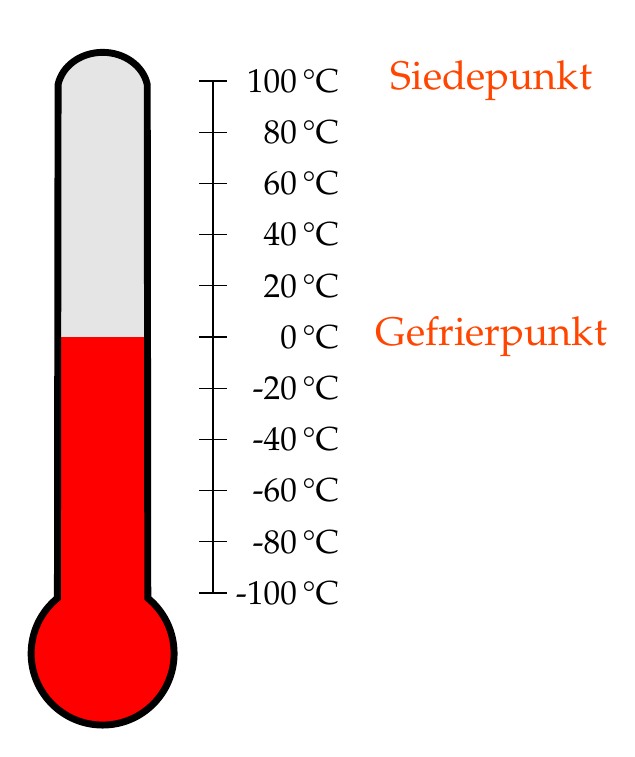
\begin{tikzpicture}[y=0.5pt, x=0.5pt,yscale=-1, inner sep=0pt, outer sep=0pt]
\foreach \y/\x in {190/100,227/90,264/80,301/70,338/60,375/50,412/40,449/30,486/20,523/10,560/0} {
  \draw (350,\y)--(370,\y) node[right](C\x) {};
  \draw node[xshift=4em,left] at (C\x) {\large \unit[\pgfmathparse{int(2*\x-100)} \pgfmathresult]{\textdegree C}~};
  }
% \foreach \u/\v in {189.999/212,231.111/192,272.222/172,313.333/152,354.444/132,395.555/112,436.666/92,477.777/72,518.888/52,559.999/32}
%     \draw (210,\u)--(190,\u) node[left](F\v){\unit[\v]{\textdegree F}};

\path[draw=black,fill=white,miter limit=4,even odd rule,line width=2.5pt,fill=gray!20]
   [thermometer][path picture={\fill[red] (C50) rectangle (path picture bounding box.south west);}];
\draw[thick] (360,190)node[yshift=4ex, OrangeRed] {} -- (360,560) ;  
% \draw (200,190)node[yshift=4ex, Cerulean] {Fahrenheit}--(200,560);
\draw node[xshift=9.5em, OrangeRed] at (C100) {\Large Siedepunkt};
% \draw node[xshift=-5em, Cerulean] at (F212) {Water boils};
\draw node[xshift=9.5em, OrangeRed] at (C50) {\Large Gefrierpunkt};
% \draw node[xshift=-5em, Cerulean] at (F32) {Water freezes};
\end{tikzpicture}
\end{document}
